\chapter{绪论}

\section{研究背景}

\subsection{半导体工艺的发展}

% (Globe Union Centralab)
% (Texas Instruments, TI)
% (Integrated Circuit, IC)
% (Fairchild Semiconductor)
1947年,贝尔实验室发明了世界上第一个晶体管,时任全球联通公司中心实验室职员的杰克·基尔比(Jack Kilby)对此产生了浓厚兴趣,并于1958年在德州仪器创造了世界上第一个采用飞线连接的锗基底扩散工艺集成电路。紧接着,仙童半导体的罗伯特・诺伊斯(Robert Norton Noyce)在1959年发明了更具有实用价值的、能够进行大规模量产的、基于导线结构的硅基底平面工艺集成电路。此后,在短短的半个世纪内,集成电路无处不在。

作为第三次工业革命的起源,集成电路的发明和应用使人类社会从工业时代迈入了信息时代,极大地解放了生产力,推动了人类社会的发展。
早在集成电路发明早期,英特尔(Intel)的创始人之一戈登·摩尔(Gordon Earle Moore)就预言半导体行业将会迅猛发展,于1965年提出了著名的摩尔定律(Moore's law)\cite{moore_law_0}:集成电路上可容纳的晶体管数目,约每隔一年翻一番(1975年修正为两年\cite{moore_law_1})。不久后,罗伯特·登纳德(Robert Heath Dennard)发现,晶体管所消耗的电压和电流,会随着晶体管的尺寸做相同比例的减少,功率密度保持不变,这便是著名的登纳德缩放定律(Dennard scaling)\cite{dennard_scaling}。登纳德定律表明,由于单位面积的晶体管的功耗维持稳定,而计算能力会随着每一代工艺节点而提升,芯片将会越来越节能。

近现代的数十年间,半导体制造商一直遵循着摩尔定律,不断缩小晶体管的尺寸,改进晶体管的制造方法%
\IfStrEq{\Version}{Open}{%
    \footnote{\url{http://www.wecorp.com.cn/newsdetail.asp?newsid=152}}。
}{。}
在传统的硅平面工艺被发明40年后,晶体管的栅极长度已经缩小到了100纳米(Nanometer, nm)以下\cite{90nm_uniaxial_strained},由于短沟道效应(Short-channel effects)的影响\cite{short-channel_effect}和工作电压的下降,载流子的界面散射加剧,迁移率降低,器件的驱动电流减小,响应速度变差。为了改善晶体管的开关特性,工业届各家厂商于2003年-2005年在90nm-65nm节点陆续引入了锗应变调控方法\cite{90nm_ge_strained,65nm_strained},实现了迁移率的大幅提升。之后,晶体管中电子的量子隧穿效应引起的漏电流问题取代了性能问题,成为了首要考虑事项,为了降低发热,高介电常数金属栅极技术(High-k Metal Gate, HKMG)被Intel于2007年在45nm工艺节点采用\cite{45nm_hkmg},改进后被再次应用在32nm节点\cite{32nm_hkmg_2nd}。后来,为了进一步降低功耗,半导体制造厂商于2012年左右陆续在22nm及以下制程全面转向由加州大学伯克利分校胡正明教授研发的鳍式场效应晶体管(Fin Field-Effect Transistor, FinFET)\cite{FinFET},延续了摩尔定律。然而,随着新工艺节点的不断推出,最新的量产工艺已经由台积电(Taiwan Semiconductor Manufacturing Company, TSMC)推进到了3nm,FinFET晶体管几乎达到了物理极限,摩尔定律陷入停滞。

\subsection{计算机体系结构的发展}

% (Clock frequency)
一方面,半导体制造厂商在不断地更新工艺制程以提高晶体管的密度;另一方面,芯片设计厂商也持续地从体系结构层面进行优化,以更好地利用额外增多的晶体管,改善芯片的性能、功耗和面积(Performance-Power-Area, PPA)。在登纳德定律的指导下,早期的集成电路设计厂商孜孜不倦地提高芯片的时钟频率,实现性能更高的单核处理器。英特尔甚至在2000年就豪言要在2011年将其生产的中央处理器(Central Processing Unit, CPU)推进至10GHz(Gigahertz)。然而,随着晶体管尺寸的持续缩小,电子的量子隧穿效应(Quantum tunneling effect)开始显露,晶体管的漏电流不断增加,功耗不减反增,登纳德定律开始失效,人们无法再简单地通过增加芯片的时钟频率来提高单核芯片的性能。同时,人们意识到,更高的时钟频率并不一定会带来芯片性能的增强。在1986年-2002年左右,伴随着主频提升的指令级并行(Instruction Level Parallelism, ILP)技术是提高处理器性能的主要方法。然而,过深的流水线会导致分支预测(Branch prediction)出错时需要花费巨大的代价来恢复状态,平白浪费许多能量,带来不可忽视的性能损失\cite{new_golden}。
同时,虽然单核处理器性能每年以50\%的速度进行提升,但内存性能的提升每年仅约7\%,这导致了冯·诺依曼结构(Von Neumann architecture)\cite{von_arch}下严重的内存墙问题(The memory wall problem)\cite{memory_wall},考虑到内存访问所需要的时间远大于CPU的计算时间,盲目提升处理器主频的作用非常有限。
另外,随着互联网的快速发展,应用的类型从传统的计算密集型向数据密集型转变,这一方面使控制流变得不规则,导致难以有效利用ILP技术提升性能,另一方面导致了大量的数据搬移,加剧了内存墙问题带来的负面影响%
\IfStrEq{\Version}{Open}{%
    \footnote{\url{https://blog.51cto.com/echo1937/1294895}}。
}{。}
最后,芯片互连线延迟所占比例的持续上升和设计复杂度的不断增加也迫使研究人员停止开发更高速的单核处理器,转而将目光朝向多核架构的研究\cite{free_lauch_over}。
如图\ref{50yrs_processor_trend}所示\cite{50yrs_processor_trend},以2005年英特尔放弃研发4GHz的奔腾四(Pentium IV)处理器为标志,多核设计开始兴起\cite{计算机体系结构基础}。

\begin{figure}[htb]
    \centering
    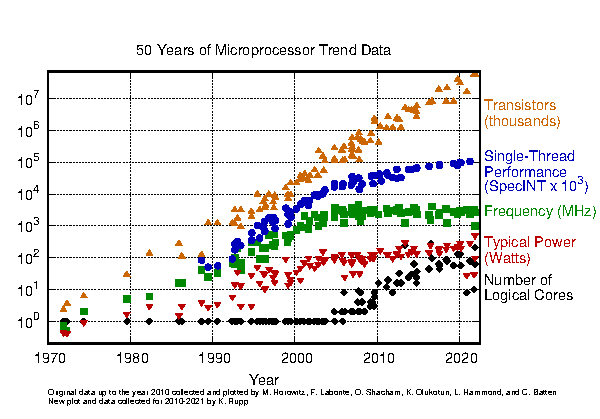
\includegraphics[width=\textwidth]{figs/50-years-processor-trend.pdf}
    \caption{近50年处理器发展趋势图}
    % \caption{近50年处理器发展趋势图\protect\footnotemark}
    \label{50yrs_processor_trend}
\end{figure}

多核架构的处理器拥有多个核心,能够同时运行多个任务,或者并行处理一个任务,大大缩短软件的运行时间。表面上看,不断增加芯片的核心数便能不断提高其处理能力,然而,多核处理器的运算能力并不能随着核数无限提升,原因如下:(1) 由于功耗墙(The power wall)的存在,即使制造出一个拥有许多个核心的芯片,也无法允许所有核心同时运行\cite{dark_silicon},这部分不工作的晶体管被称为“暗硅(Dark silicon)”;(2)在阿姆达尔定律中\cite{amdahl_law},任务在多核处理器下的理论加速比为:
\begin{equation}
    \label{amdahl_law}
    \text{加速比} = \frac{W_s+W_p}{W_s+ \frac{W_p}{p}}
\end{equation}
式中$W_s$和$W_p$为任务规模中的串行分量(不能被并行的部分)和并行分量(可以被并行的部分),可见加速比上限由任务中不能被并行处理的部分决定,若程序没有并行分量,那么不论使用多少核的处理器,任务都无法被加速;(3)由于内存提升的速度远小于处理器提升的速度,导致内存墙问题越来越严重,对某些应用来讲,盲目堆砌多核,不但不能加速任务的处理,反而导致了性能的下降\cite{multicore_bad}。

为了解决多核架构遇到的问题,软件和硬件人员分别从两方面入手进行优化。一方面,与多核处理器配套的软件如操作系统和编译器等工具开始充分发展,尽可能利用多核架构的优点,提高任务的运行速度;另一方面,计算机体系结构人员开始采用不同的方法来解决“暗硅”问题和内存墙问题。对于内存墙问题,研究人员使用多级缓存(Multi-level caches)结构和更先进的分支预测方法来增加cache的命中率;对于“暗硅”问题,学术界和工业界提出了3个方法来充分利用未工作的晶体管\cite{is_dark_silicon}:(1)低速多核。把处理器中每个核的运行频率限制在一个较低的水平,充分利用处理器的并行性,提高运算能力,例如英特尔设计的采用太阳能供电的x86多核处理器\cite{solar_x86};(2)自动超频。允许多个核心在短时间内达到很高的频率用来处理高计算量的任务,之后迅速将每个核心的频率降低来减缓发热,常用于由电池供电的对功耗有严格要求的芯片;(3)专用集成电路。利用ASIC性能高、发热低的优点,把“暗硅”部分设计成专用加速器,将CPU和ASIC结合,提高整体的处理能力。
为了得到能效更高的处理器,设计人员往往结合多种方法进行优化,比如英特尔的睿频技术(Turbo Boost Technology)\cite{intel_turbo_boost},ARM的大小核架构(big.LITTLE)\cite{arm_big_little}等。发展到现代,广义的处理器已经不仅仅是一个只有传统运算核心的芯片,而是成为了一个包含许多专用处理单元如GPU(Graphics Processing Unit)、NPU(Neural Processing Unit)、ISP(Image Signal Processor)、嵌入式FPGA(embedded FPGA, eFPGA)、DSP(Digital Signal Processing)等模块的复杂异构片上系统(System on Chip, SoC)。

随着机器学习(Machine Learning, ML)的飞速发展,人工智能(Artificial Intelligence, AI)模型对算力的需求激增。在2012年之前,训练一个ML系统所需的算力大约每17到29个月翻一番\cite{AI:computing_demand_trend},增长率和摩尔定律保持一致。然而,2012年杰弗里·辛顿(Geoffrey Everest Hinton)的学生亚历克斯·克里泽夫斯基(Alex Krizhevsky)设计了AlexNet\cite{AI:AlexNet}这一8层卷积神经网络(Convolutional Neural Network, CNN),利用GPU夺得了ImageNet LSVRC(Large Scale Visual Recognition Challenge)竞赛的冠军,并大幅领先第二名10.8个百分点,掀起了CNN研究的热潮,深度学习(Deep Learning)迎来了大爆发。伴随着互联网的快速发展和全球社会数字化转型带来的海量数据,深度学习常规模型(Regular-scale Model)训练一次所需的算力大约每4-9个月翻一番\cite{AI:computing_demand_trend}。同时,随着2016年以谷歌(Google)的AlphaGo\cite{AI:AlphaGo}战胜韩国棋手李世石为代表,大规模模型(Large-Scale Model)开始引领人工智能的潮流,计算量大约每9到10个月翻一番\cite{AI:computing_demand_trend}。如此巨大的算力需求和不断改变的算法模式是传统的运算芯片所无能为力的,于是各种领域专用架构(Domain-Specific Architecture, DSA)竞相涌现,牺牲了部分的通用性,实现了高能效计算,如寒武纪的DianNao\cite{Accelerator:DianNao}、Google的TPU(Tensor Processing Unit)\cite{Accelerator:TPU}、GraphCore的IPU(Intelligence Processing Unit)\cite{Accelerator:IPU}、华为的DaVinci架构\cite{Accelerator:DaVinci}、百度的昆仑芯片\cite{Accelerator:Kunlun}等,计算机体系结构迎来了新黄金时代\cite{new_golden}。与ASIC相比,DSA的通用性更强,能够适应日新月异的AI算法。
同时,CPU、GPU和FPGA架构也不断革新,引入了各种针对ML应用的专用处理单元,如Intel至强(Xeon)处理器中的AI加速单元\cite{Accelerator:intel_xeon_4th}、英伟达(Nvidia)GPU中的张量计算核心(Tensor Core)\cite{Accelerator:nvdia_h100_tensor_core_4th}、赛灵思(Xilinx)FPGA中的AI引擎(AI Engine, AIE)\cite{Accelerator:amd_versal_AIE}。

与计算机视觉(Computer Vision, CV)领域不同,在自然语言处理(Natural Language Processing, NLP)方面,纯粹由注意力机制构成的Transformer模型\cite{AI:attention_is_all}取代了CNN,占据了主导地位。在Google提出Transformer模型一年后,大规模语言模型(Large Language Model, LLM)开始出现,以OpenAI旗下的GPT(Generative Pre-trained Transformer)为代表,LLM的大小一直在飞速增长:2018年发布的GPT-1参数量为1.17亿,数据量为5GB(Gigabyte);2019年发布的GPT-2参数量为15亿,数据量为40GB;2020年发布的GPT-3参数量为1750亿,数据量增加到45TB(Terabyte)。研究表明,Transformer类模型训练所需的运算量每2年增加750倍,远超摩尔定律的演进速率,如图\ref{AI:ai_and_compute}所示\cite{ai_and_memory_wall}。

\begin{figure}[htb]
    \centering
    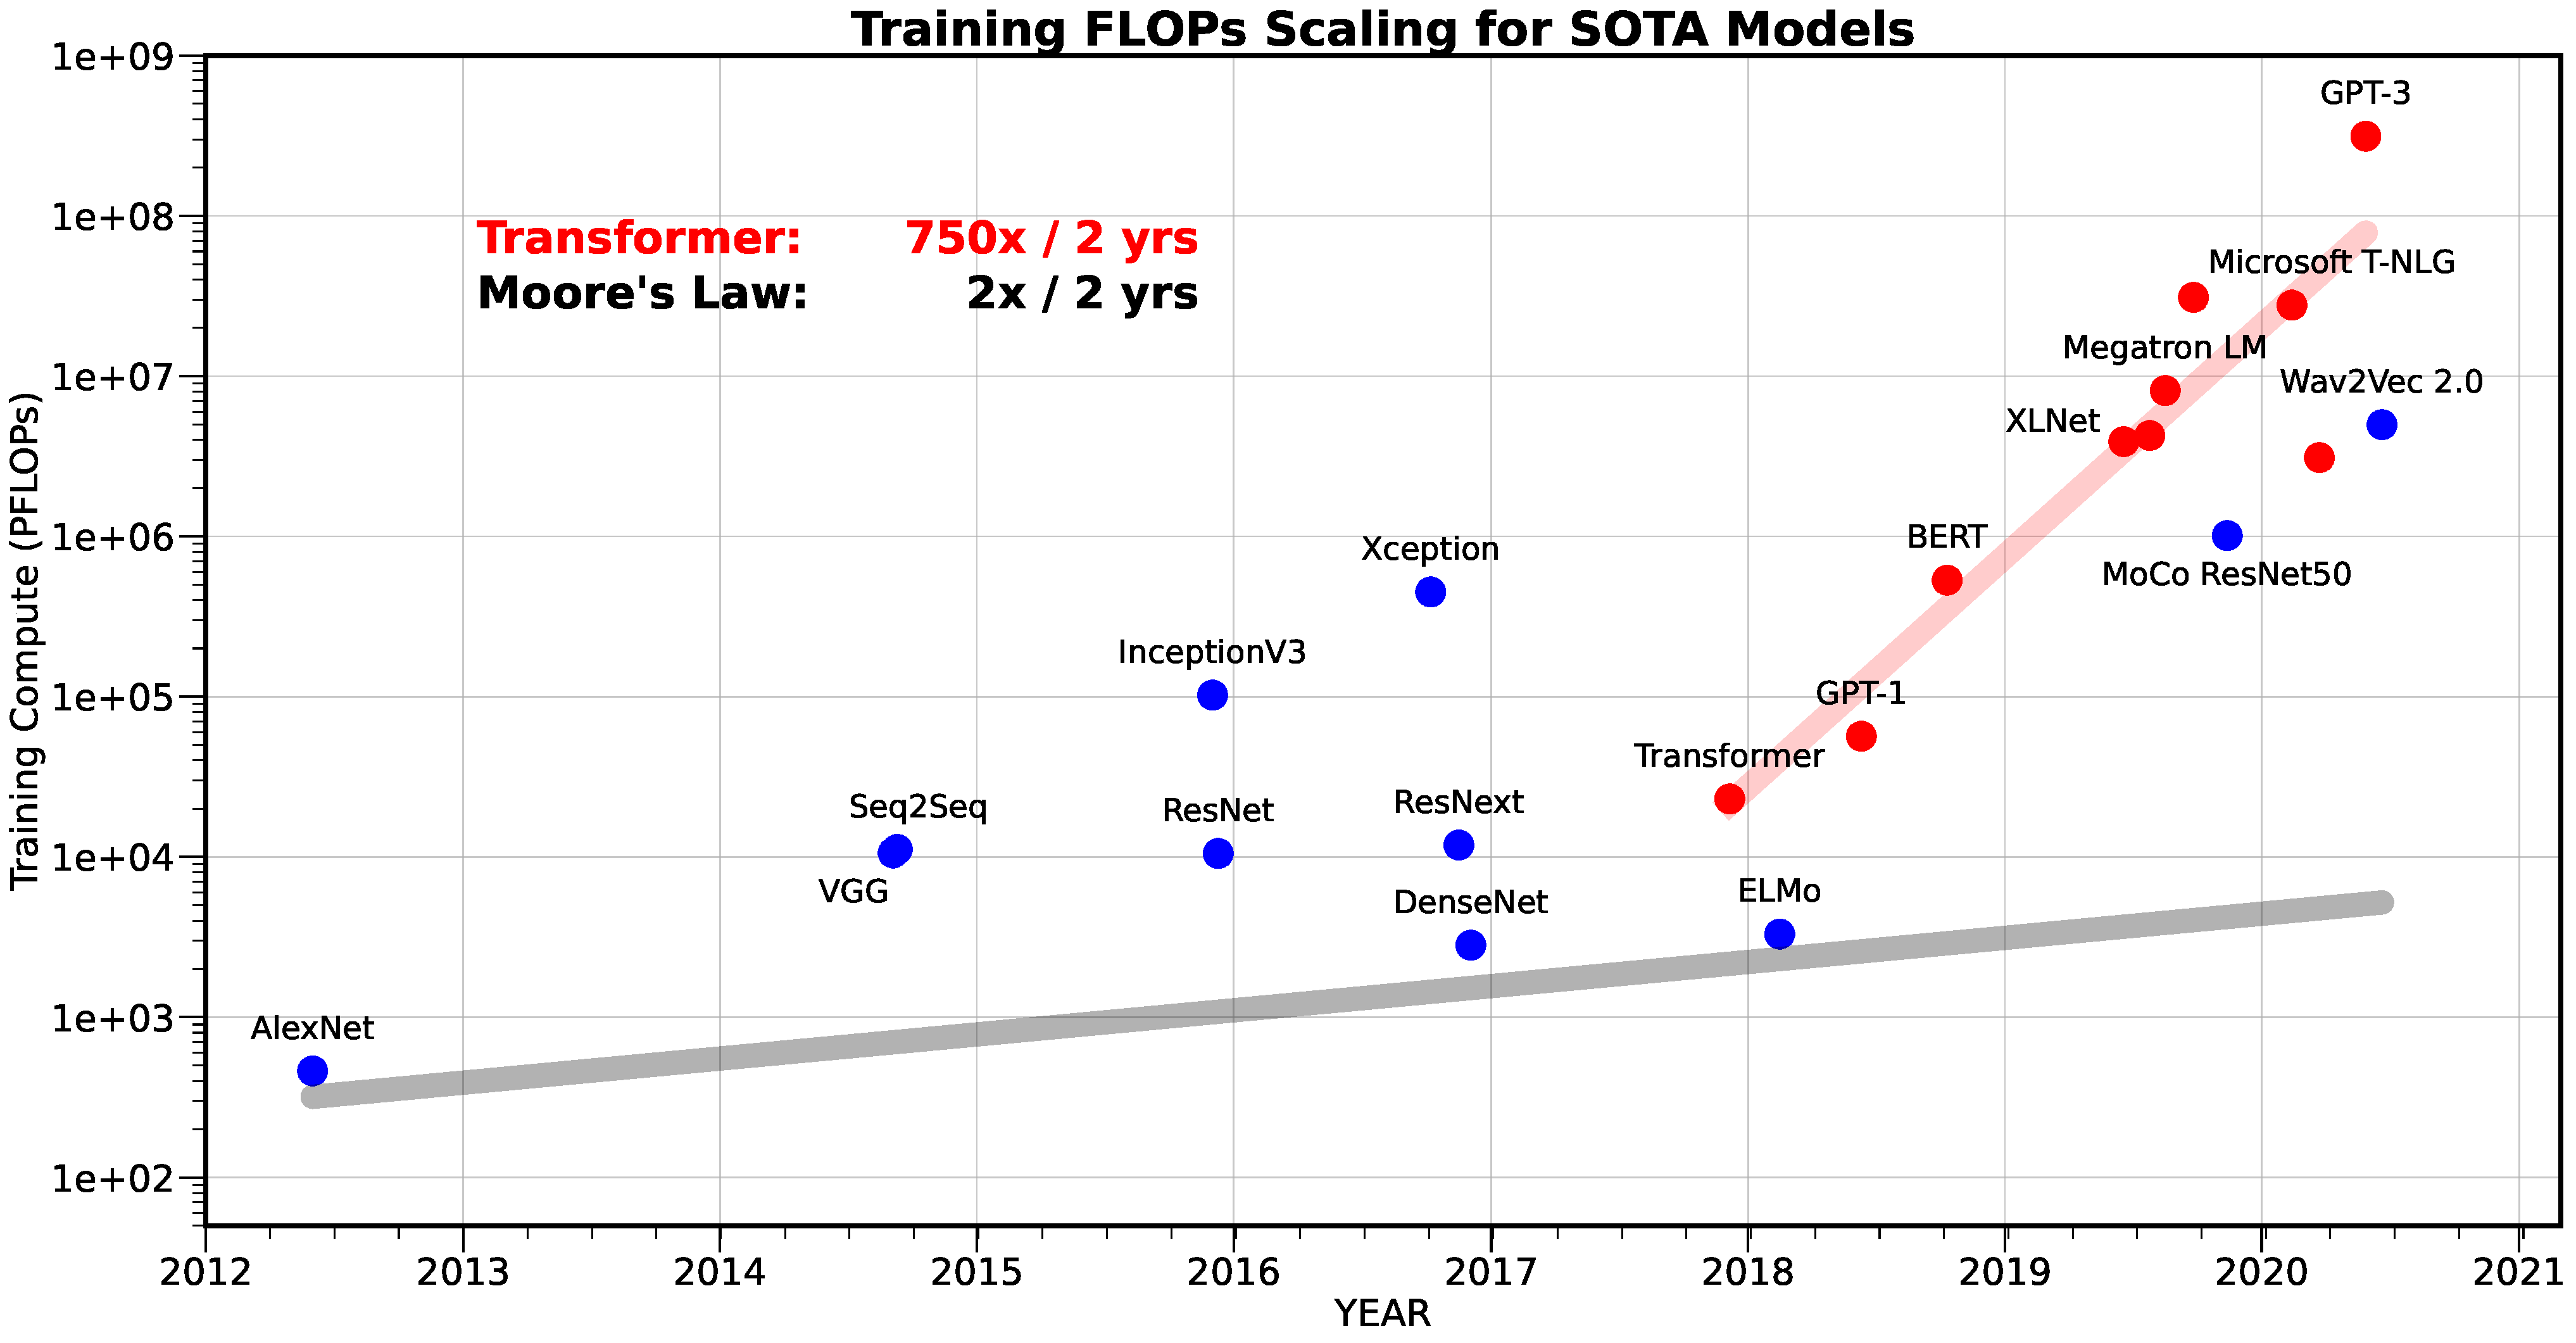
\includegraphics[width=\textwidth]{figs/AI-Fig-ai_and_compute.pdf}
    \caption{Transformer类模型训练所需的运算量}
    \label{AI:ai_and_compute}
\end{figure}


如此巨大的计算需求,需要海量的算力进行支撑。目前业界通用的办法是利用并行化技术在多个GPU或DSA上进行训练,以求在合理的时间内获得想要的结果。然而,这会伴随着资源的大量消耗。例如,训练一个GPT-3模型需要355个GPU年(一块GPU运行355年的运算量),花费460万美元,耗电1287兆瓦时(Megawatt Hour, MWh),大约相当于120个家庭1年的用电量\cite{AI:carbon_google_2021,AI:zeus}。并且,训练阶段的能耗通常只占模型整个生命周期的40\%\cite{AI:carbon_google_2022},ChatGPT的火热导致这一占比对GPT类应用更低,这产生了大量碳排放,对环境造成了很大的负担。为了降低能耗,研究人员从算法和硬件两方面来对AI应用进行优化。一方面,高效的ML模型架构可以在更少计算量的情况下实现更高的精度,减少资源的消耗;另一方面,采用专门用于AI训练和推断的芯片能够提高系统的能效,实现绿色计算(Green Computing)\cite{AI:green_computing}。但是,目前的研究表明,LLM模型的规模越大,往往NLP任务的效果越好,\cite{AI:llm_overview},这意味着模型的精简程度十分有限。同时,芯片的能效提升远远跟不上模型的规模增长,人们迫切需要新的方法在提升算力的同时降低资源消耗。


\subsection{后摩尔时代的技术路线}

以生成式AI(Generative AI)为代表的人工智能等应用的发展,对半导体材料和器件提出了更高的要求。当前,随着硅晶体管的演进接近物理极限,不仅特征尺寸的缩小越来越困难,迭代产生的工艺红利也消失殆尽,硅基电子技术临近生命周期极限。为了探索集成电路领域新的发展规律,持续提高芯片能效,学术界和工业界提出了多个发展方向,这里列举几个典型的技术路线%
\IfStrEq{\Version}{Open}{%
    \footnote{\url{https://irds.ieee.org/editions/2022}}:
}{:}

(1)More Moore\cite{more_moore}

“More Moore”即“深度摩尔”,其基本思路是延续摩尔定律的发展,在兼顾性能和功耗的同时,继续缩小晶体管的尺寸。随着FinFET的漏电越发严重,对沟道拥有更强控制能力的全环栅晶体管(Gate All Around FET, GAAFET)将成为未来的主流\cite{GAA}。

(2)More than Moore\cite{more_than_moore}

“More than Moore”即“超越摩尔”,侧重于功能的多样化,由应用需求驱动,通过先进封装技术实现异质集成系统。与不断优化晶体管的“More Moore”路线不同,“More than Moore”从需求端出发,以系统应用为起点,尝试在提高芯片集成度和能效的同时降低芯片制造的成本。在SoC中,除了逻辑(Logic)和存储(Dynamic Random Access Memory, DRAM)部分以外,模拟(Analog)、射频(Radio Frequency, RF)等模块往往并不能随着工艺的迭代获得显著地性能改善,甚至可能会变差。因此,数字(Digital)部分可由先进工艺实现,而其余部分可选择更合适的工艺进行流片,最后不同模块通过先进封装技术组合在一起,模块间通过高速接口进行通讯,实现整体的能效提升。


(3)Beyond Complementary Metal Oxide Semiconductor(CMOS)\cite{beyond_cmos}

前面两种路线仍然是基于硅基集成电路进行拓展,“Beyond CMOS”是指利用CMOS之外的新器件、新材料来制造晶体管,提高芯片的能效。与CMOS相比,这类新器件往往具有更高的密度、更强的性能、更低的功耗,但可能还无法大规模制造或制造成本不能接受。目前,该方向是学术界和工业界研究的热点之一,各种新型方案百花齐放,比如低功耗的隧穿场效应晶体管(Tunneling FET, TFET)\cite{TFET}、与CMOS工艺兼容的单电子晶体管(Single Electron Transistor, SET)\cite{SET}、具有高迁移率的石墨烯晶体管(Graphene Transistor)\cite{Graphene_transistor}、适合RF电路的碳纳米管场效应晶体管(Carbon Nanotube FET, CNFET)\cite{Carbon_Nanotube_FET}等。但是,这一方向的绝大多数成果还未走出实验室,仍处于初期的前瞻性研究阶段,距离商业化较远。

\section{研究意义}

\subsection{近似计算与容错应用} \label{approximate_computing_advance}

随着人工智能的不断发展,计算需求急剧增加,带来大量的能源消耗。同时,在可穿戴设备、便携设备和数据中心等场景,集成电路面临的功耗问题日益严峻,人们需要寻找新的芯片设计方法以同时满足高性能和低功耗的严苛要求。
在实际生活中,许多应用具有错误容忍的特性,这类应用被称为容错应用(Error-tolerant applications)。一个典型的例子是,当观看视频时,由于感知的限制,即使视频中某些帧出错甚至丢失了,人类很可能也察觉不到。类似地,即使搜索引擎返回的结果没那么精确,查询者也可以接受。
近似计算(Approximate computing)是一种新型的计算范式(Paradigm),与精确计算(Exact computing)相比,它可能返回不准确的结果。与容错应用结合,近似计算可以在满足精度需求的前提下节省大量能源,达到降低功耗、提高能效的目的。
因此,在数字信号处理、机器学习等场景中,近似计算得到了工业界和学术界的广泛关注\cite{AC:survey:survey's_survey,AC:survey:hanjie_2013_ETS}。

目前,有关近似计算的研究主要集中在四个层面:

(1)软件层近似(Software-level approximation)

软件层的近似有多种实现方式,比如在循环中跳过一些迭代来更快地获得计算结果,或者根据条件语句进行判断,从而跳过某些任务的执行来减少程序运行时间。另外,许多启发式算法(Heuristic algorithm)如模拟退火(Simulated annealing)和遗传算法(Genetic algorithm)常常需要在一定的时间内获得次优解(Sub-optimal solution),也属于软件层近似的一种。

(2)近似电路(Approximate circuits):

通过对加法器(Adder)\cite{AC:Aadd:simple_yet}、乘法器(Multiplier)\cite{AC:AM:Adapt}、除法器(Divider)\cite{AC:Div:2019dac}等算术运算单元(Arithmetic units)引入近似,获得能效的提升,被称为电路级近似。电路级近似的实现方式大体上可以分为两类:电压调节(Voltage scaling)和功能近似(Functional approximation)\cite{AC:ALS:survey}。其中,电压调节是通过降低模块的工作电压但不降低频率来减少电路的功耗。然而,这一般会产生时序错误(Timing error),带来难以控制的计算误差\cite{AC:Arith:overscale}。功能近似通常聚焦在电路结构或门级网表(Gate-level netlist)的简化上,与电压调节相比,功能近似的方法带来的误差易于控制,也是目前近似计算研究最为深入的方向\cite{AC:Arith:survey_hanjie}。

(3)近似存储和近似内存(Approximate storage and memory):

与存储精确数据相比,存储近似后的数据能够改善数据读取的延迟,降低数据搬移的能耗。例如,通过舍弃浮点数(Floating-point number)低有效位(the Least Significant Bit, LSB),可以减少数据存储所需要的位宽(Bit width),提高存储密度。在基于Flash的固态硬盘(Solid State Drive, SSD)中引入近似计算可以提高SSD的读取性能\cite{AC:Store:ASCache}。对于内存或cache来说,降低DRAM的刷新率\cite{AC:Store:DRAM}或静态随机存储器(Static Random-Access Memory, SRAM)\cite{AC:Store:SRAM}的供电电压也可以达到节省功耗的目的。

(4)近似系统(Approximate system):

对不同子模块如传感器、内存、处理器、通信接口等进行协同优化的方法被称为近似系统,与单独优化各个组件相比,近似系统能够取得更好的效果\cite{AC:Sys:camera}。

\subsection{近似乘法器的优势}

乘法(Multiplication)是科学计算中十分常见的一种操作,也是许多AI应用中最消耗资源的部分\cite{AC:AM:Overfit}。在计算机发展的早期,由于芯片集成度较低,并没有专门用来直接完成乘法的硬件,而是将其拆分为逻辑与、加法和移位,利用算术逻辑单元(Arithmetic Logic Unit, ALU)来实现,这种乘法方式被称为移位加\cite{计算机体系结构基础}。ALU在一个时钟周期内只能对一个部分积进行加法运算,速度较慢,随着摩尔定律的不断发展,集成电路可容纳的晶体管越来越多,现代处理器中已经有专门的硬件来完成乘法,速度大大提高。
作为数字电路系统中一个能够实现两个数相乘的运算电路,乘法器已经被研究了几十年,其性能和功耗依赖于设计的电路结构。
% (见\ref{精确乘法器})。

为了提高如图像处理(Image processing)、数据挖掘(Data mining)、多媒体技术(Multimedia technology)、深度学习等许多容错类应用的计算效率,人们提出了近似乘法器的概念,与精确乘法器相比,近似乘法器(Approximate multiplier)通常具有更小的面积、更低的延迟、更优的功耗,但在某些情况会输出不正确的结果。
利用近似乘法器对应用中被频繁调用的乘法操作在硬件上进行优化,一方面能够提高处理速度、减少资源消耗,另一方面又不会带来明显的输出质量下降。

\subsection{近似乘法器与逻辑综合}

不同方法得到的近似乘法器往往具有不同的精度和硬件开销,直观上看,工程师可以根据需要直接把一个大型设计中的精确乘法器替换为性能较优的近似乘法器以期得到更好的PPA。然而这种直接替换的方法存在一定的局限性。事实上,基于硬件成本较低的近似乘法器实现的大型设计在整体上并不一定有优势,原因如下:大型设计中的乘法器单元并不是独立存在的,而是会与别的电路产生连接,逻辑综合工具在运行过程中会使用大量的启发式算法对整个设计进行优化,由于不同近似乘法器单元在设计中与电路连接后具有不同的拓扑结构,生成不同的优化空间(比如一个近似乘法器在单独评估时所有输入的到达时间均假设为0,但在设计中与电路结合后却并非如此),所以存在这样一种可能,即硬件成本较低的近似乘法器在与一些电路结合后整体上变得难以优化,导致整个设计的PPA不占优势。

因此把具有不同质量的近似乘法器组合在一起,形成一个乘法器库,在逻辑综合时调用库中符合精度要求的不同近似乘法器单元对精确乘法器进行替换并对整个电路进行评估,选择电路整体性能最优时对应的乘法器(存在该乘法器是精确乘法器的可能)进行后续的物理实现,与直接根据近似乘法器的硬件开销进行替换相比,能够实现更好的PPA。这种方法被称为近似逻辑综合。


\section{国内外研究现状}

\subsection{近似乘法器研究现状}

近似电路的设计通常聚焦在功能近似层面\cite{AC:ALS:survey},近似乘法器也不例外。
有关近似乘法器在功能近似层面的研究大致可分为3个阶段:早期(2011年-2016年),研究人员通常采用手工的方法修改电路的晶体管结构\cite{AC:AM:IMPACT}或逻辑函数\cite{AC:AM:KMap},以达到提升性能的目的,但这种方法费时费力、效率较低,且生成的乘法器的质量难以保证;之后,有关近似乘法器的研究转到了自动化方法,以2016年基于笛卡尔遗传规划的设计方法为代表\cite{AC:AM:CGP_2016},伴随着数学转换方法\cite{AC:AM:OU}和近似电路综合\cite{AC:ALS:ALSRAC},利用非手工的方法生成近似乘法器的研究开始成为主流;在2018年之前,有关近似乘法器的研究多数集中在以逻辑门为基础的AISC电路上,从2018年开始,有研究人员发现既有的面向ASIC的近似乘法器无法在FPGA上取得同等程度的性能提升,于是开始有工作基于手工修改查找表编码的方式设计专门面向FPGA的近似乘法器,取得了良好的效果\cite{AC:AM:FPGA:SMApproxLib}。

\subsection{逻辑综合研究现状}

广义的逻辑综合可分为传统逻辑综合、精确逻辑综合(Exact logic synthesis)和近似逻辑综合三类。
其中,传统逻辑综合(通常简称为逻辑综合)在整个芯片设计流程中处于最上游的位置,是指将数字电路的高抽象级描述(通常是指寄存器传输级),在功能一致的前提下经过布尔函数化简、优化后,转换到的逻辑门级别的网表的过程,其性能对芯片最终的面积和延迟起决定性作用。
目前有关逻辑综合研究主要集中在优化及映射算法的开发、改进\cite{LS:Narrowing}和命令序列的探索上\cite{LS:Bulls-Eye},有工作表明目前学术界开源工具的FPGA综合性能已不弱于工业界\cite{LS:Narrowing}。
精确逻辑综合(可简称为精确综合)要求在给定的约束下找到电路的最佳实现,比如基于给定的门的种类和数量上限对布尔网络进行映射\cite{LS:exact_syn},属于传统逻辑综合中的一个细分研究方向。
近似逻辑综合包括两个方向,一个方向侧重于近似算术单元的生成,也被叫做近似电路综合;另一个方向更靠近传统逻辑综合,即基于已有的近似库对大型设计进行优化和映射,该方向也是本文的研究内容之一。

% 下面对传统的逻辑综合方向的研究现状做一些介绍。

\subsection{近似逻辑综合研究现状}

目前有关近似逻辑综合的研究多集中在近似电路综合的方向\cite{AC:ALS:ALSRAC},但也有工作尝试将近似单元库和逻辑综合联系起来,以期对大型设计实现更好的效果,比如文献\cite{Accelerator:ALWANN}通过自动化为DNN加速器的每一层配置不同精度的近似乘法器,避免了耗时的重训练过程,实现了比单独应用一种近似乘法器更高的精度和更低的功耗。



\section{研究动机}


目前已有的近似乘法器设计方法往往假设输入是均匀分布的,然而大多数应用中乘法运算的两个操作数都是非均匀分布的,这导致生成的近似乘法器在某些应用中误差较大、性能较差。另外,近似乘法器一般是不对称的,即不满足交换律,现有的自动化生成方法并没有考虑交换输入对生成的乘法器的质量产生的影响。因此需要一种能够同时考虑数据分布(Input distribution)和输入极性(Polarity)的自动化近似乘法器设计方法,在降低乘法器误差的同时提高电路性能。

与ASIC近似乘法器相比,FPGA近似乘法器领域发展较慢。尽管已有的ASIC近似乘法器能够直接迁移到FPGA上面,但由于组合逻辑(Combinational logic)在ASIC中由逻辑门(Logic gate)和金属线(Metal wire)构成而在FPGA中由LUT和布线资源组成,因此基于ASIC实现的近似乘法器在FPGA上往往无法获得相同程度的硬件性能提升,需要专门开发面向FPGA架构的近似乘法器。
目前大多数面向FPGA的近似乘法器设计方法均采用手工修改LUT编码的方式实现。然而,这些手工设计近似乘法器的过程通常非常耗时,并且生成的乘法器之间误差和硬件性能差距很大,无法根据应用的需求进行灵活地调整,因此需要针对FPGA提出一个新的自动化设计方法,能够在短时间内生成许多具有不同精度的高质量软核(Softcore)乘法器。

最后,在得到许多高性能的近似乘法器之后,如何从逻辑综合的角度为每一个大型设计挑选出合适的用来替换精确乘法器的近似乘法器单元是一个关键的问题。


\section{本文主要工作及组织结构}

本文的主要工作集中在近似电路中高能效定点数(Fixed-point number)近似乘法器的设计及应用上。首先,针对现有的自动化ASIC近似乘法器设计方法没有同时考虑数据分布和输入极性这一不足之处,本文提出了一种基于白盒优化的能够在设计阶段同时考虑输入分布和极性(Polarity)的近似乘法器设计方法,有效降低了硬件成本,提高了电路能效。同时,针对现有ASIC近似乘法器无法在FPGA上取得同等性能收益这一特点,以及手工修改LUT编码的FPGA近似乘法器设计方法耗时且不灵活这一缺点,本文提出了一种基于贝叶斯优化的自动化FPGA近似乘法器设计方法,在短时间内能够生成大量具有不同精度的高质量近似乘法器,满足不同应用的精度需求。最后,基于得到的近似乘法器库,本文提出了一种基于MFFC自适应超图划分的强化学习逻辑优化序列探索框架,并进行了近似逻辑综合的研究。主要贡献如下:

(1)面向ASIC,提出并开源了一个白盒优化的考虑输入分布和极性的高质量自动化近似乘法器生成方法,该方法在对部分积进行累加求和之前,引入与(AND)、或(OR)、异或(XOR)和移位(Shift)操作,降低部分积的个数,实现能效的提升。具体来说,基于应用驱动,统计应用中乘法器的输入数据分布,并在考虑极性的情况下对部分积进行压缩,减轻后续的累加负担。为了能够自动化处理,将寻找较优压缩操作的问题建模成数学问题,并用 MATLAB进行求解。
基于改进的Baugh-Wooley算法\cite{EM:baugh-wooley,EM:baugh-wooley_modified_PP_reorga,EM:baugh-wooley_diff},方法经过扩展后实现了对补码有符号乘法器的支持。基于位宽为$8\times8$无符号乘法的三个不同规模的神经网络包括LeNet、AlexNet和VGG16以及位宽为$16\times16$有符号定点数乘法的有限冲击响应(Finite Impulse Response, FIR)滤波器的实验结果表明,与国际前沿工作相比,生成的近似乘法器在几乎没有精度损失的前提下,功耗延迟面积积(Product of Power, Delay, and Area, PDA)提升了26.4\%-27.1\%。

(2)面向FPGA,设计并开源了一个基于黑盒优化的近似乘法器生成器,该方法假设乘法器的部分积在生成后、累加前存在一次由半加器阵列进行的压缩操作,针对半加器,提出删减(Eliminate)、或之和(OR $Sum$)、直接进位(Direct $Cout$)、精确(Exact)四种简化方法,利用贝叶斯优化(Bayesian optimization)和详细设计的能够同时考虑硬件PPA和软件精度的目标函数($cost$ function)对半加器的优化空间进行探索,生成高质量的近似乘法器集合。与国际前沿工作中1167个近似乘法器相比,生成的乘法器综合指标平均提升28.70\%-38.47\%,且处于帕累托前沿(Pareto front)。

(3)基于前面两种自动化方法得到的ASIC和FPGA乘法器库,首先针对传统逻辑综合,提出并开源了一个基于MFFC自适应超图划分的强化学习(Reinforcement learning)逻辑优化序列探索框架。基于超过150个电路的实验结果表明,面积延迟积(Area Delay Product, ADP)比ABC\cite{LS:ABC} resyn2平均提高了5.17\%。

(4)将本文提出的框架与本文生成的近似乘法器库结合,对基于不同近似乘法器实现的DNN加速器进行了研究,结果显示近似乘法器的单独硬件成本提升与对应加速器的硬件成本提升存在一定偏差。

\begin{figure}[!htb]
    \centering
    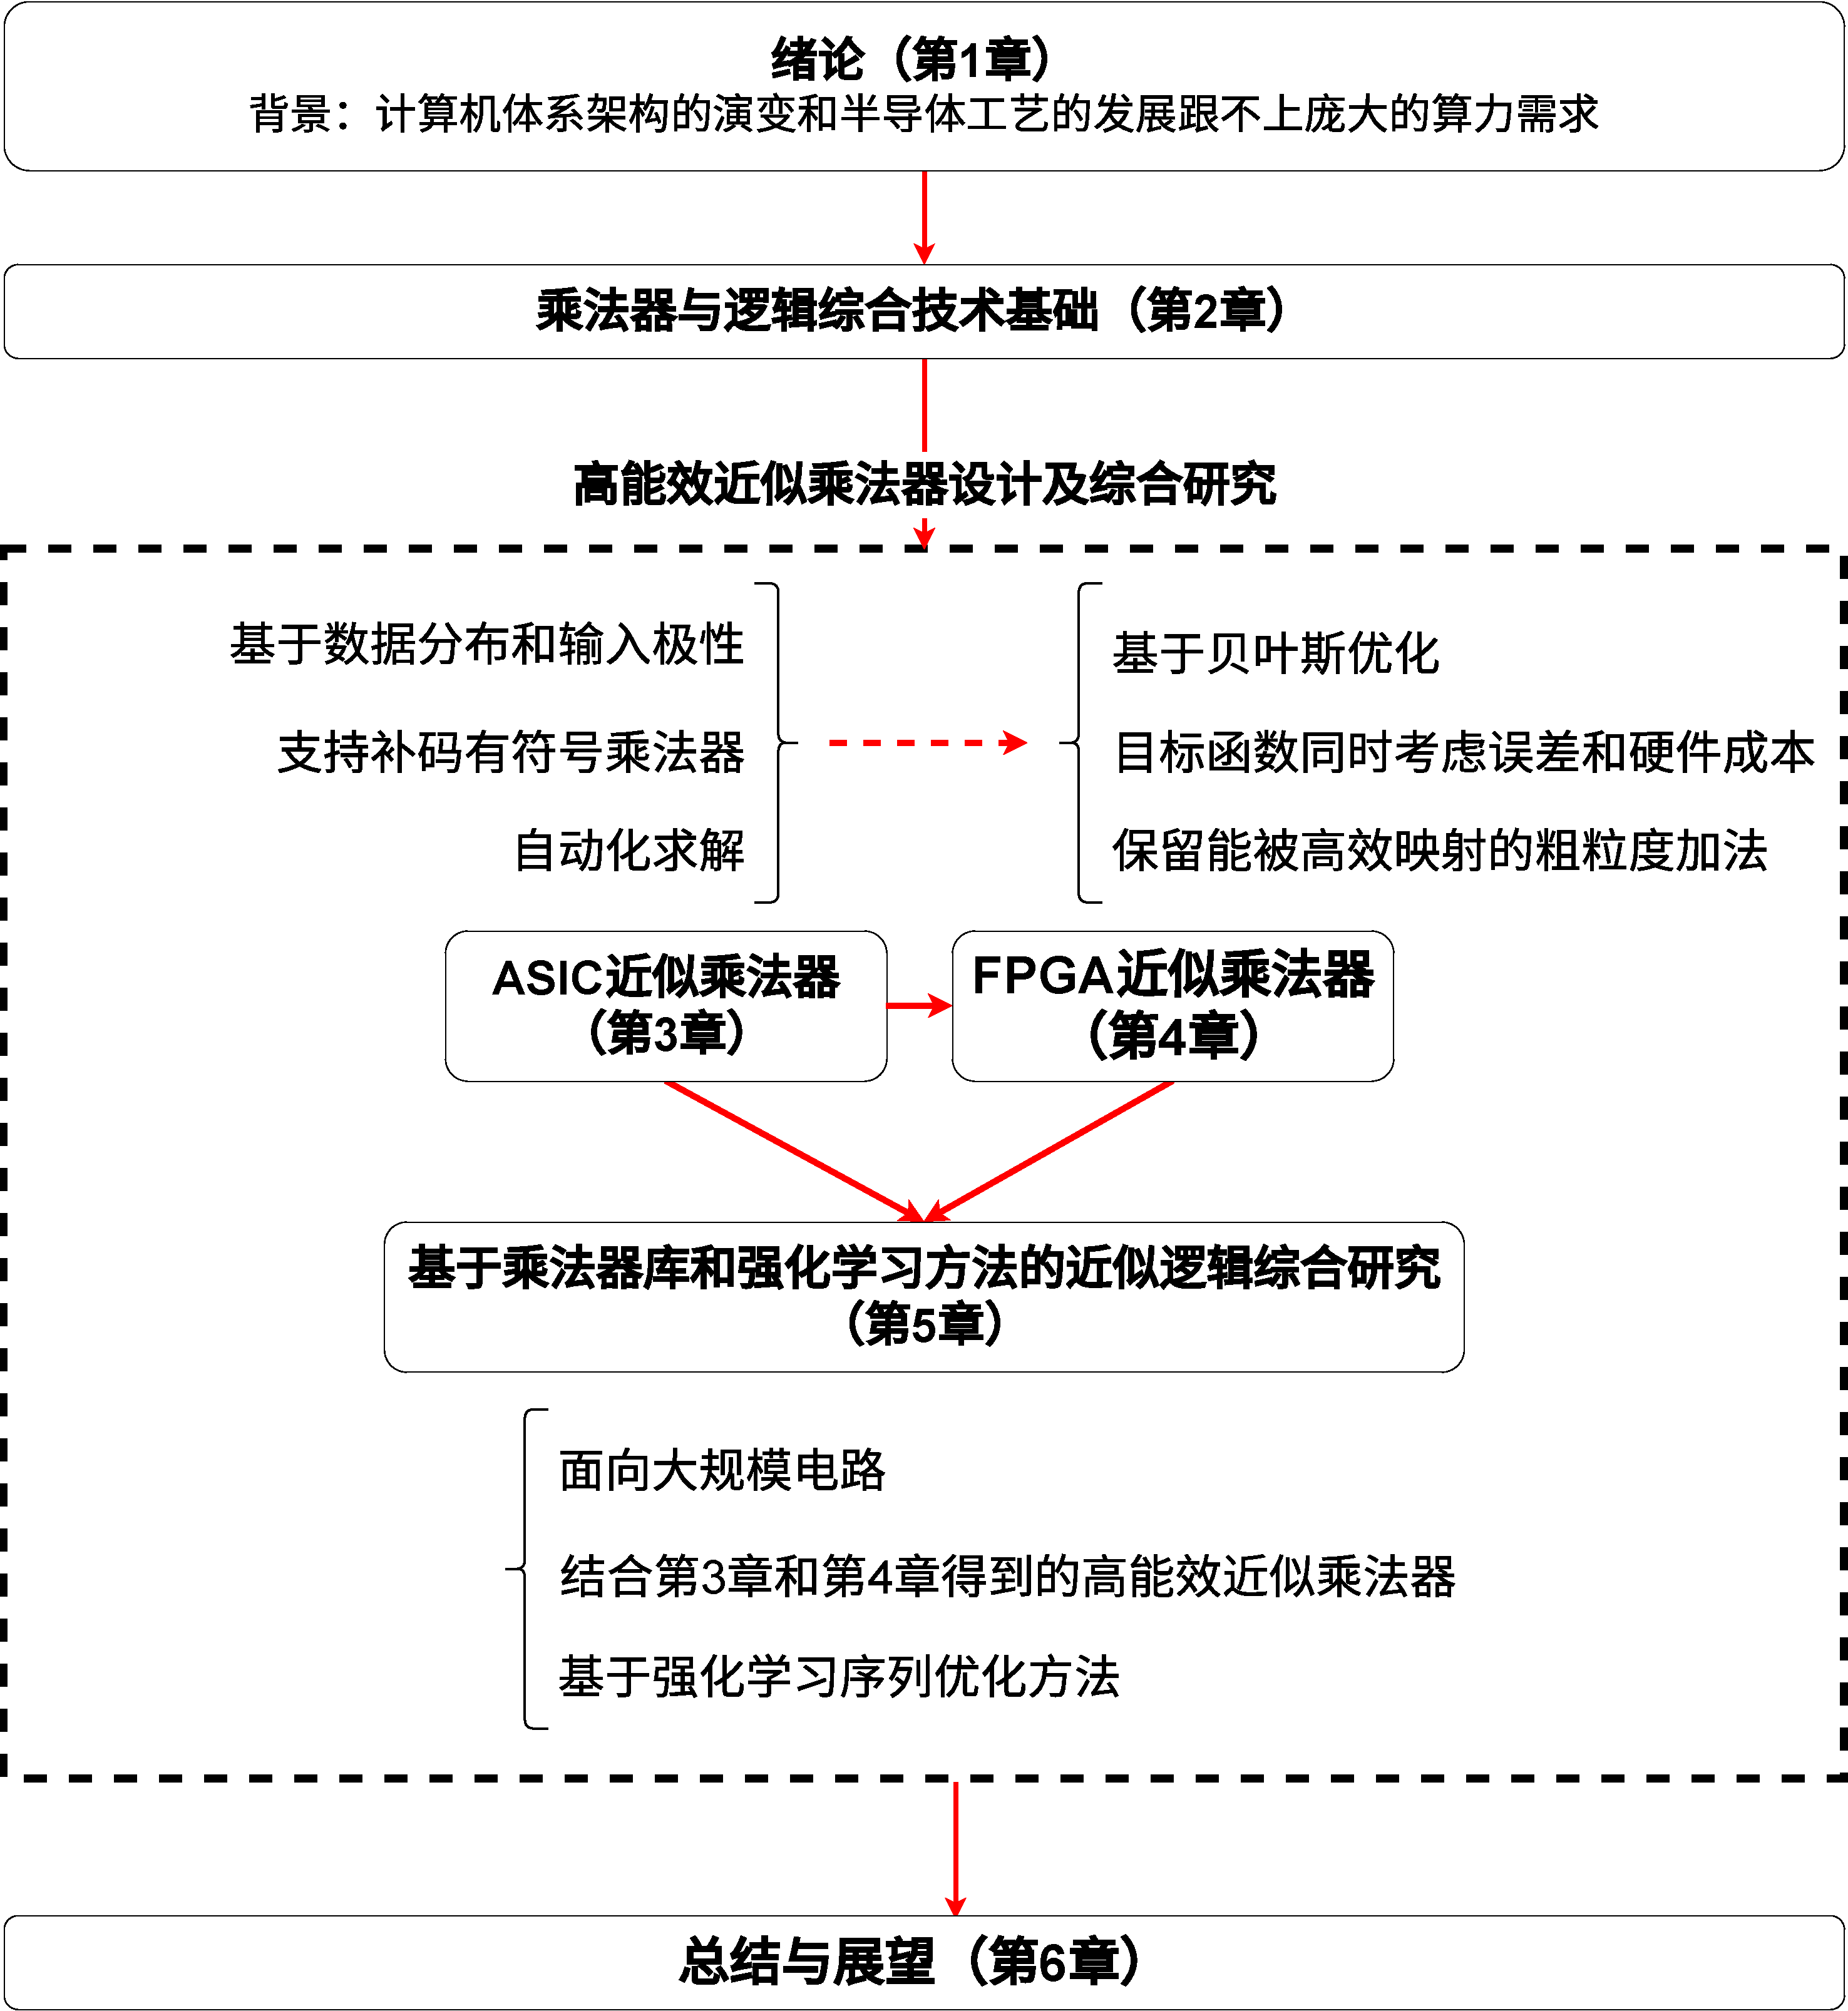
\includegraphics[width=\textwidth]{figs/论文结构.pdf}
    \caption{本文组织结构}
    \label{本文组织结构}
\end{figure}

本文共有六个章节,整体框架如图\ref{本文组织结构}所示,各章节的组织结构安排如下:

第一章,绪论。首先介绍了自集成电路发明以来半导体工艺和计算机体系结构的发展,之后分析了近似计算具有的优势以及国内外相关工作的研究现状,引出本文的研究目的。

第二章基于乘法器库的近似逻辑综合技术基础。首先介绍了精确定点数乘法器的运算过程及不同的实现方法,以及采用Mitchell近似的对数乘法器\cite{EM:mitchell};之后阐述了目前主流的衡量近似电路(主要是算术单元)误差的指标以及不同近似乘法器的设计方法;最后介绍了逻辑综合的相关内容。

第三章,ASIC近似乘法器设计。首先介绍了数据分布和输入极性对乘法器精度的影响,接着介绍了基于白盒优化的考虑数据分布和输入极性的自动化近似乘法器设计方法,并与国际前沿工作进行对比。

第四章,FPGA近似乘法器设计。首先对比了已有的近似乘法器在ASIC和FPGA上的性能差异,接着提出了基于黑盒优化的自动化近似乘法器生成器,并与国际前沿工作进行误差和硬件开销比较。

第五章,逻辑综合研究。设计并实现了一个基于MFFC自适应超图划分的强化学习逻辑优化序列探索框架,并与已有的序列优化方法进行对比,基于超过 150个电路的实验结果显示,与 ABC 的脚本 resyn2 相比,面积延迟积平均提高了5.17\%。

第六章,将提出的逻辑优化框架与近似乘法器库结合,探究基于不同近似乘法器对DNN硬件加速器带来的影响。

第七章,总结与展望。该章节总结了本文的主要研究工作和成果,分析了工作中存在的局限性,并对未来进一步的探索方向进行了展望。

